%%%%%%%%%%%%%%%%%%%%%%%%%%%%%%%%%%%%%%%%%%%%
%
%   A Beamer presentation by Rodrigo Platte, Arizona State University, May 18 2007.
%   Feel free to modify this file to generate your own presentation.
%
%   This Latex file should be compiled with pdflatex, for this reason, it is recommended 
% that you convert the figures in your presentation to pdf. Postscript files (.ps and .eps) 
% will not compile properly when pdflatex is used. You may use commands like "convert"
% or "eps2pdf" (in linux) to convert your figures. 
%
%   The final output is a PDF file that is best visualized with Adobe Reader.
%
%   More information can be found in beameruserguide.pdf
%
%   This presentation requires the following files:
%   BEAMERoptions.tex, ASUlogo.pdf,  asu.pdf, beamerouterthememathASUlogo.sty
%  intro1.pdf, intro2.pdf, intro3.pdf, intro4.pdf, analytic.pdf
%%%%%%%%%%%%%%%%%%%%%%%%%%%%%%%%%%%%%%%%%%%%


\documentclass[compress]{beamer}
% Use this instead for printing and distributing your slides (suppresses overlays)
%\documentclass[handout]{beamer}


%%%%%%%%%%%%%%%%%%%%%%%%%%%%%%%%%%%%%%%%
% Edit the file BEAMERoptions.tex to change theme, color, fonts, logo, etc.%
%%
%% Generated by Rodrigo Platte, Arizona State University, May 18 2007 %%
%% Edit this file to change how your presentation looks!
%%
%% For more information, please read the manual: beameruserguide.pdf
%%	 

% Select a theme
%%%%%%%%%%%%%%%%%%%%%%%%%%%
   % \usetheme{Frankfurt}
  % \usetheme{Singapore}
   % \usetheme{Madrid}
   % \usetheme{Antibes}
   % \usetheme{Berkeley}
   \usetheme{default}
%%%%%%%%%%%%%%%%%%%%%%%%%%%

% Select a color theme
%%%%%%%%%%%%%%%%%%%%%%%%%%%
  % \usecolortheme{seagull}
  % \usecolortheme{crane}
  \usecolortheme{default}
  % \usecolortheme[rgb={.4,0,0}]{structure} % Red colors
    % \usecolortheme[rgb={.2,0,0}]{structure} % Dark Red colors
  %\usecolortheme[rgb={.6,.5,.2}]{structure} % Yellow/Green colors
%%%%%%%%%%%%%%%%%%%%%%%%%%%
  
 % Select a font theme
 %%%%%%%%%%%%%%%%%%%%%%%%%%
    \usefonttheme{structurebold}
   %  \usefonttheme{structuresmallcapsserif}
   % \usefonttheme{structureitalicserif}
      % \usefonttheme{serif}
 %%%%%%%%%%%%%%%%%%%%%%%%%%

 % Select a background color  
 %%%%%%%%%%%%%%%%%%%%%%%%%%%%%%
   %\setbeamertemplate{background canvas}[vertical shading][bottom=white,top=gray!30]
   % \setbeamertemplate{background canvas}[vertical shading][bottom=white,top=red!10!black!30]
   %\setbeamertemplate{background canvas}[vertical shading][bottom=white,top=green!20!black!30]
   % \setbeamertemplate{background canvas}[vertical shading][bottom=white,top=white]
%%%%%%%%%%%%%%%%%%%%%%%%%%%%%%%

% Select a color for math text
%%%%%%%%%%%%%%%%%%%%%%%%%%%%%%% 
% \setbeamercolor{math text}{fg=red!80!black}
%%%%%%%%%%%%%%%%%%%%%%%%%%%%%%%


% This command suppresses the navigation symbols at footline
% comment the command below if you  want navigation symbols 
%\setbeamertemplate{navigation symbols}{}

% Set the size of the font in frame title
\setbeamerfont{frametitle}{size=\normalsize}


% This command will generate a gray footline with the ASU logo in
% each frame
  % \useoutertheme{mathASUlogo}


					                                         %
%%%%%%%%%%%%%%%%%%%%%%%%%%%%%%%%%%%%%%%%

% Load packages
%%%%%%%%%%%%%%%%%%%%%
\usepackage[english]{babel}
\usepackage{graphics}
\usepackage{multimedia} % for movies and sound
\usepackage{times}
\usepackage{subfigure}

% \usepackage{movie15}

%%%%%%%%%%%%%%%%%%%%%
\definecolor{darkgreen}{rgb}{0,0.4,0}

%% The title and name 
%% Note: [short title]{long title}, [short author(s) name]{long author(s) name}
\title[Data-driven neural field modelling]{Data-driven neural field modelling}
\author[Dean R. Freestone]{\emph{Dean R. Freestone} \\ \tiny{Supervisors: David B. Grayden, Anthony N. Burkitt, Levin Kuhlmann and Mark J. Cook}}
% , Parham Aram, Michael Dewar, Kenneth Scerri, David B. Grayden, Visaken Kadirkamanathan} }
\date[]{02-11-2011}
% Show ASU logo in title page
%%%%%%%%%%%%%%%%%%%%%%
\institute[The University of Melbourne]{

\includegraphics[height=2.5cm]{./Figures/LOGOs.pdf} \\
{BEI, SVHM, UoM (DEEE)}}
% \institute[University of Sheffield]{
% {Department of Automatic Control and Systems Engineering}}


%%%%%%%%%%%%%%%%%%%%%




%%%%%%%%%%%%%%%%%%%%%%%%%%%%%%%%%%%%%%%%%%
%%%%%%%%%%%% Presentation Starts Here %%%%%%%%%%%%%%%%
%%%%%%%%%%%%%%%%%%%%%%%%%%%%%%%%%%%%%%%%%%


\begin{document}

%%% Title frame %%%%%
\begin{frame}[plain]
	\titlepage
	\transboxout
\end{frame}

\begin{frame}
\begin{center}
	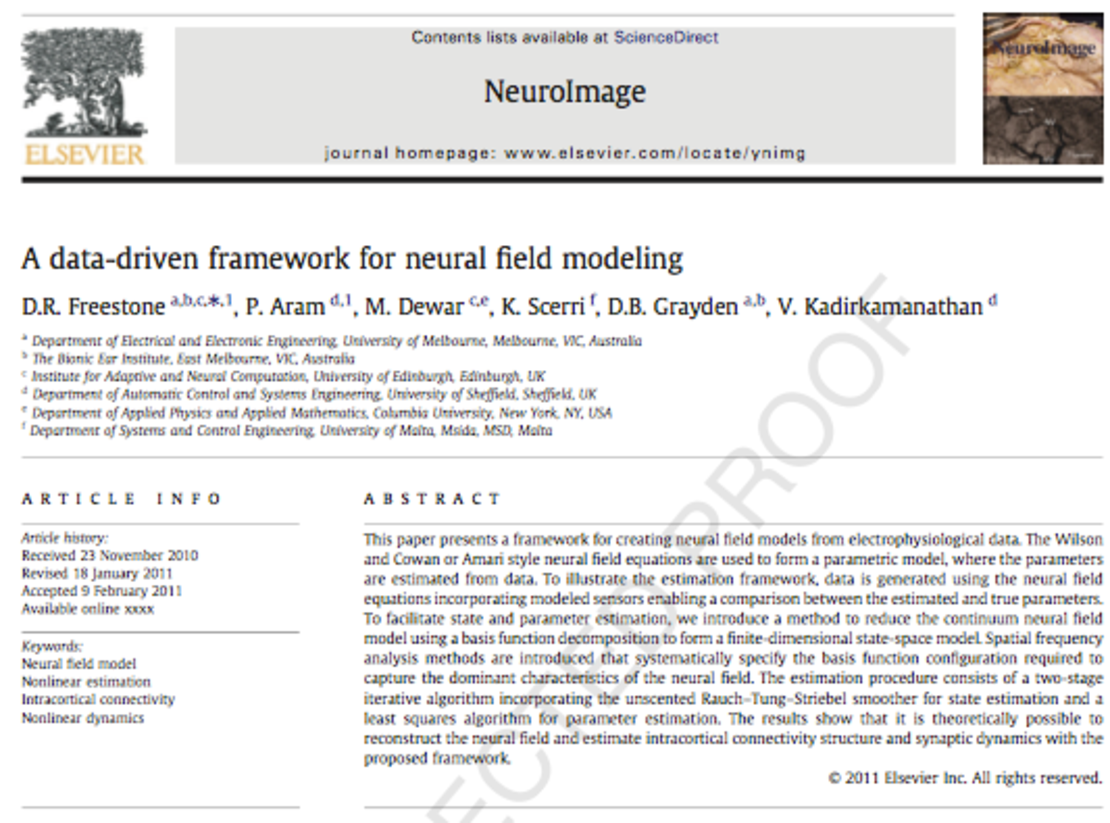
\includegraphics[height=8cm]{./Figures/PaperSceenShot.pdf} 
\end{center}
% \begin{picture}(.1,.1)
% 	\put(40,100){\includegraphics[height=2cm]<2-4>{./Figures/Parham.pdf}}
% 	\put(90,100){\includegraphics[height=2cm]<3-4>{./Figures/Mike.pdf}}
% 	\put(140,100){\includegraphics[height=2cm]<4>{./Figures/Ken.pdf}}
% \end{picture}
\end{frame}

%%%% Outline (optional) %%%%%%%%%%%%%%%%%%%%%
%% The outline depends on \section and \subsection commands
%%%%%%%%%%%%%%%%%%%%%%%%%%%%%%%%%%
\begin{frame}
  \frametitle{Outline}
  \tableofcontents[pausesections]
  % \transboxin
\end{frame}
%%%%%%%%%%%%%%%%%%%%%%%%%%%%%%%%%%

\section[Introduction]{Introduction}

\subsection{Why data-driven modelling}

\begin{frame} \frametitle{Motivation}
	\begin{picture}(0,0)
	% \put(-60,-150){\includegraphics<1>[height=10cm]{./Figures/InterictaliEEGA4.pdf}}
	\put(-60,-150){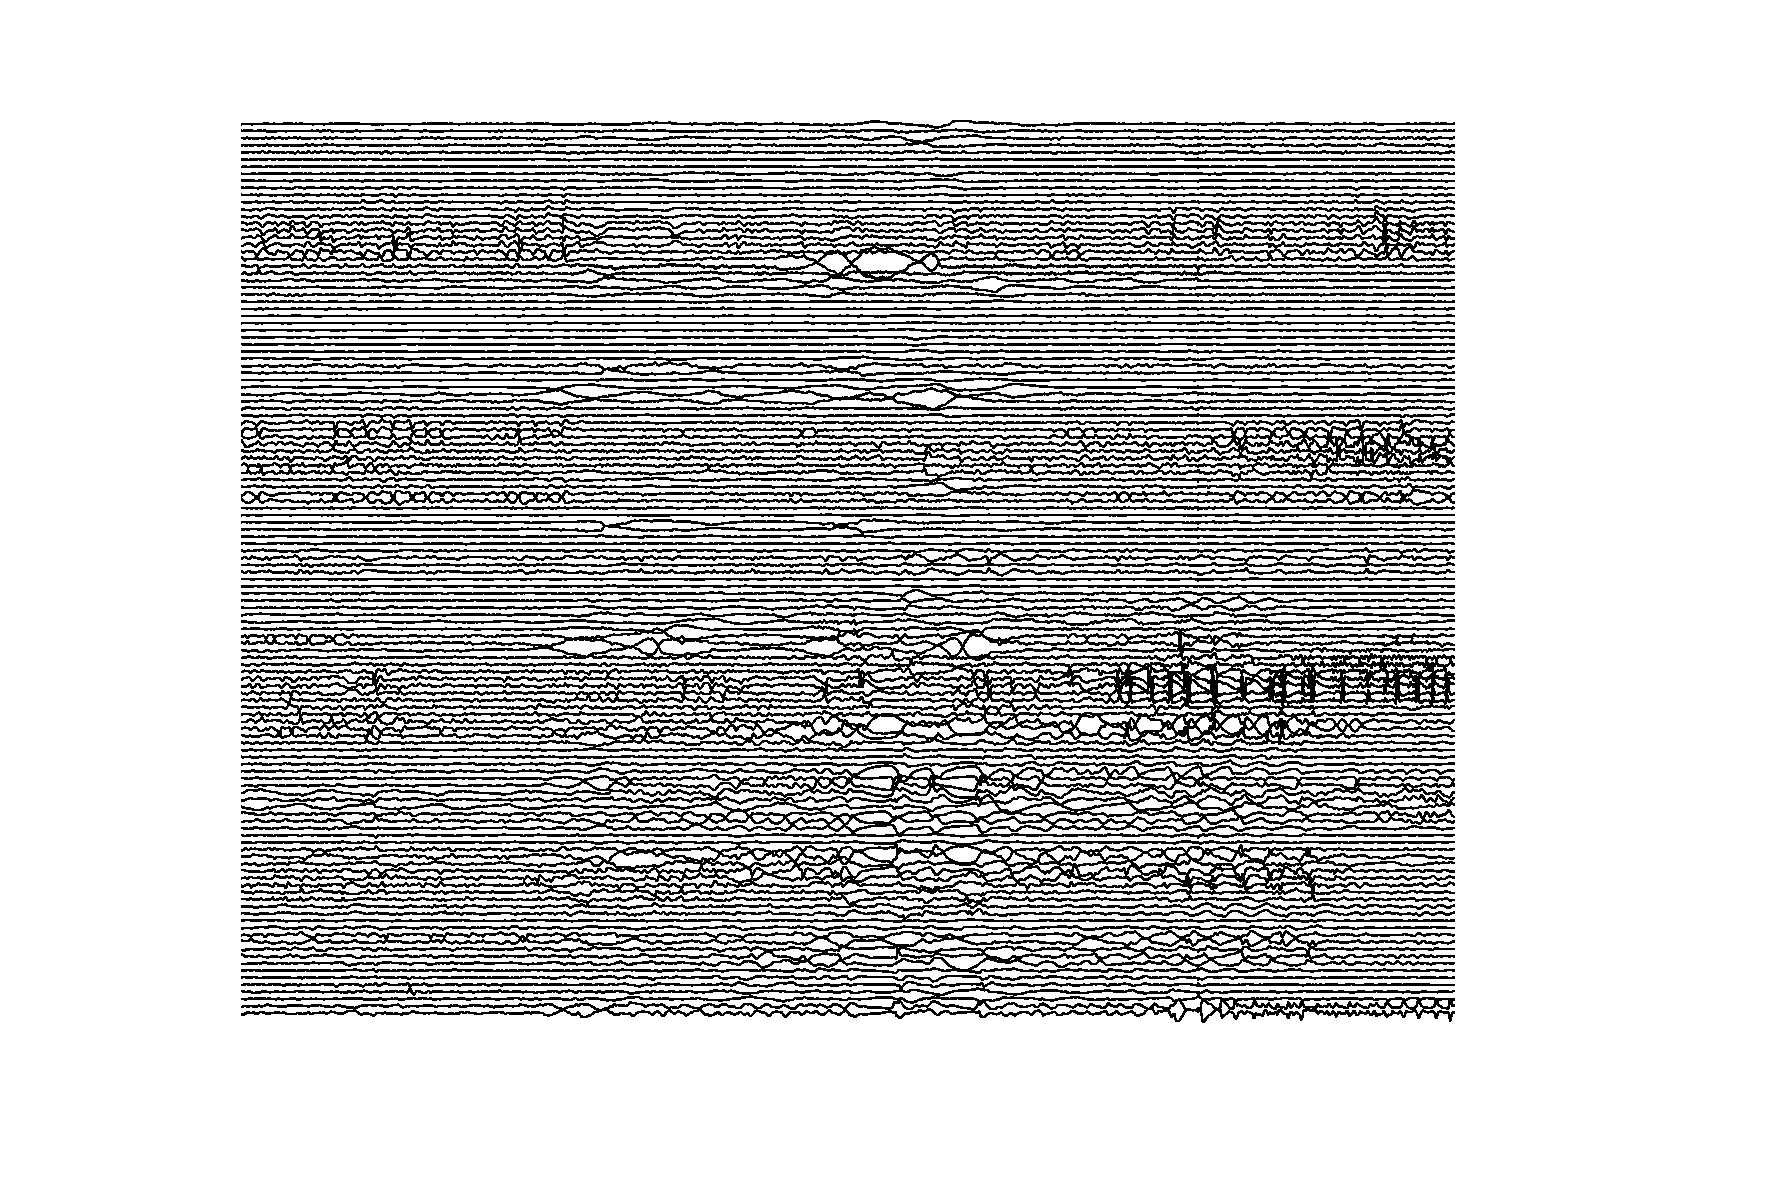
\includegraphics[height=10cm]{./Figures/StartIctaliEEGA4.pdf}} 
	% \put(-60,-150){\includegraphics<3>[height=10cm]{./Figures/IctaliEEGA4.pdf} }
	% \put(-60,-150){\includegraphics<4>[height=10cm]{./Figures/PostIctaliEEGA4.pdf}} 
	\end{picture}
\end{frame}

\begin{frame}\frametitle{Electrical stimulation as therapy}
	\begin{center}
		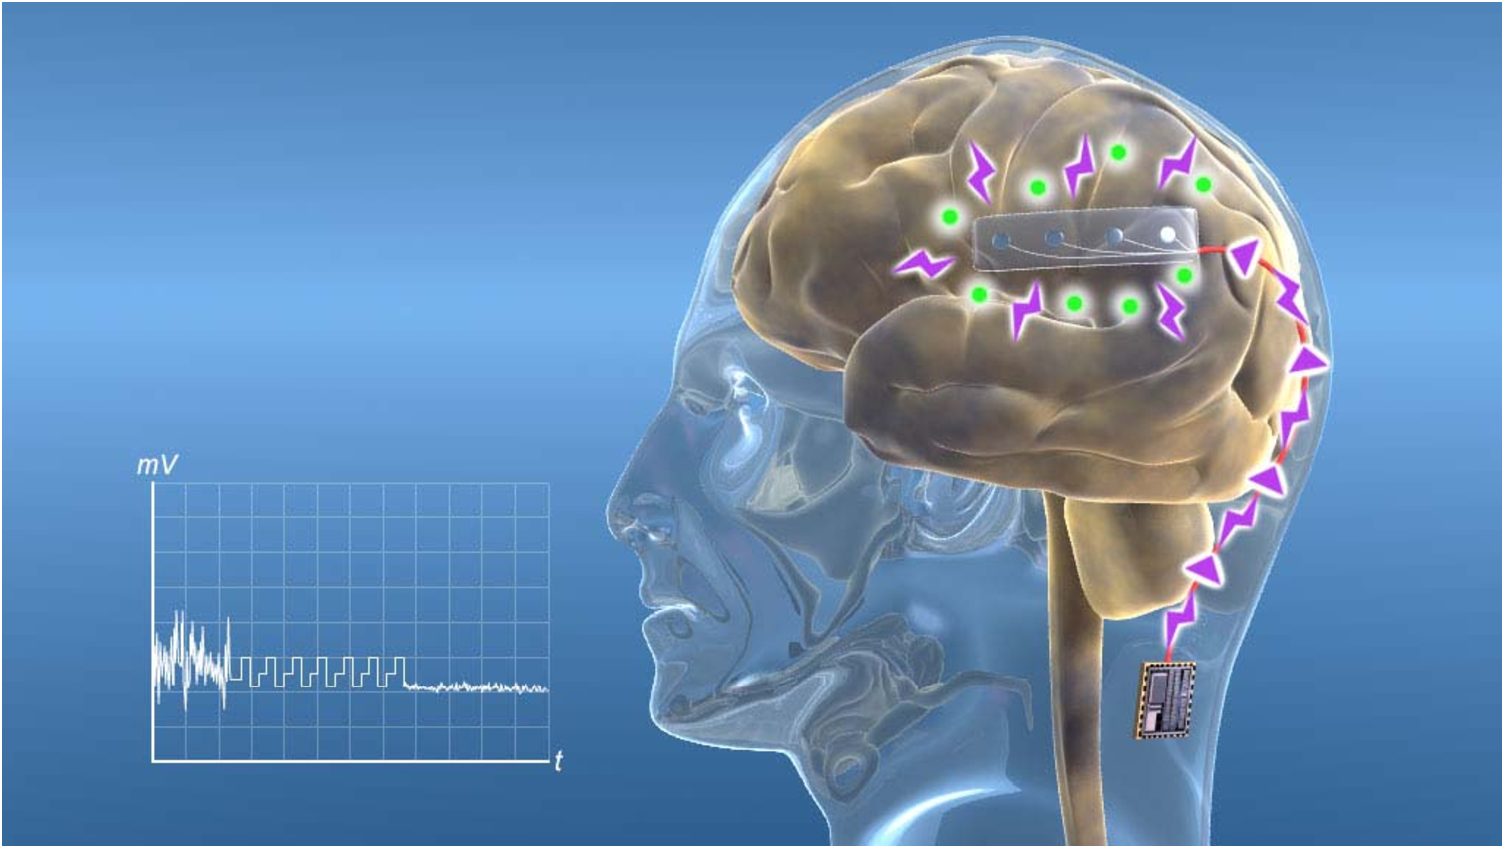
\includegraphics[height=6cm]{./Figures/ExampleTherapyStim.pdf} 
	\end{center}	
\end{frame}

\begin{frame}\frametitle{Trial and error (open loop) stimulation strategy}
	\begin{center}
		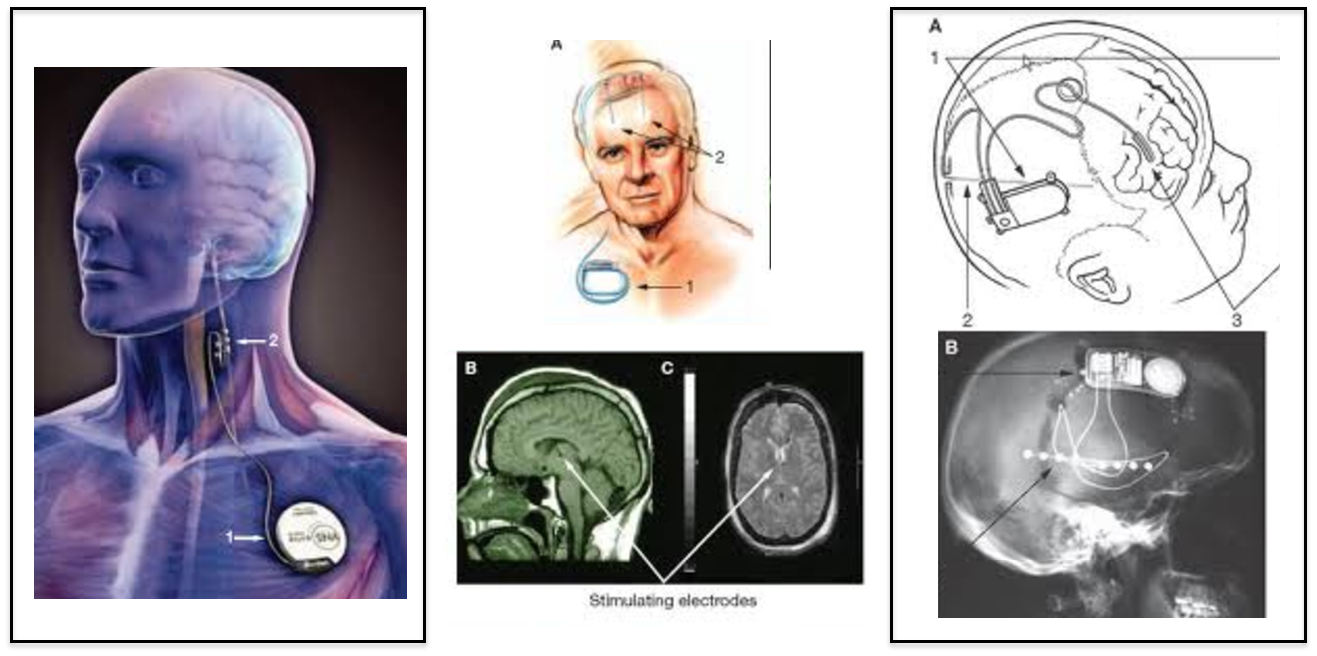
\includegraphics[height=5cm]{./Figures/EpilepsyStimulators.pdf} 
	\end{center}
	Parkinson's (persistent) vs. epilepsy (intermittent)	
\end{frame}

\begin{frame}\frametitle{Inception}
	\begin{center}
		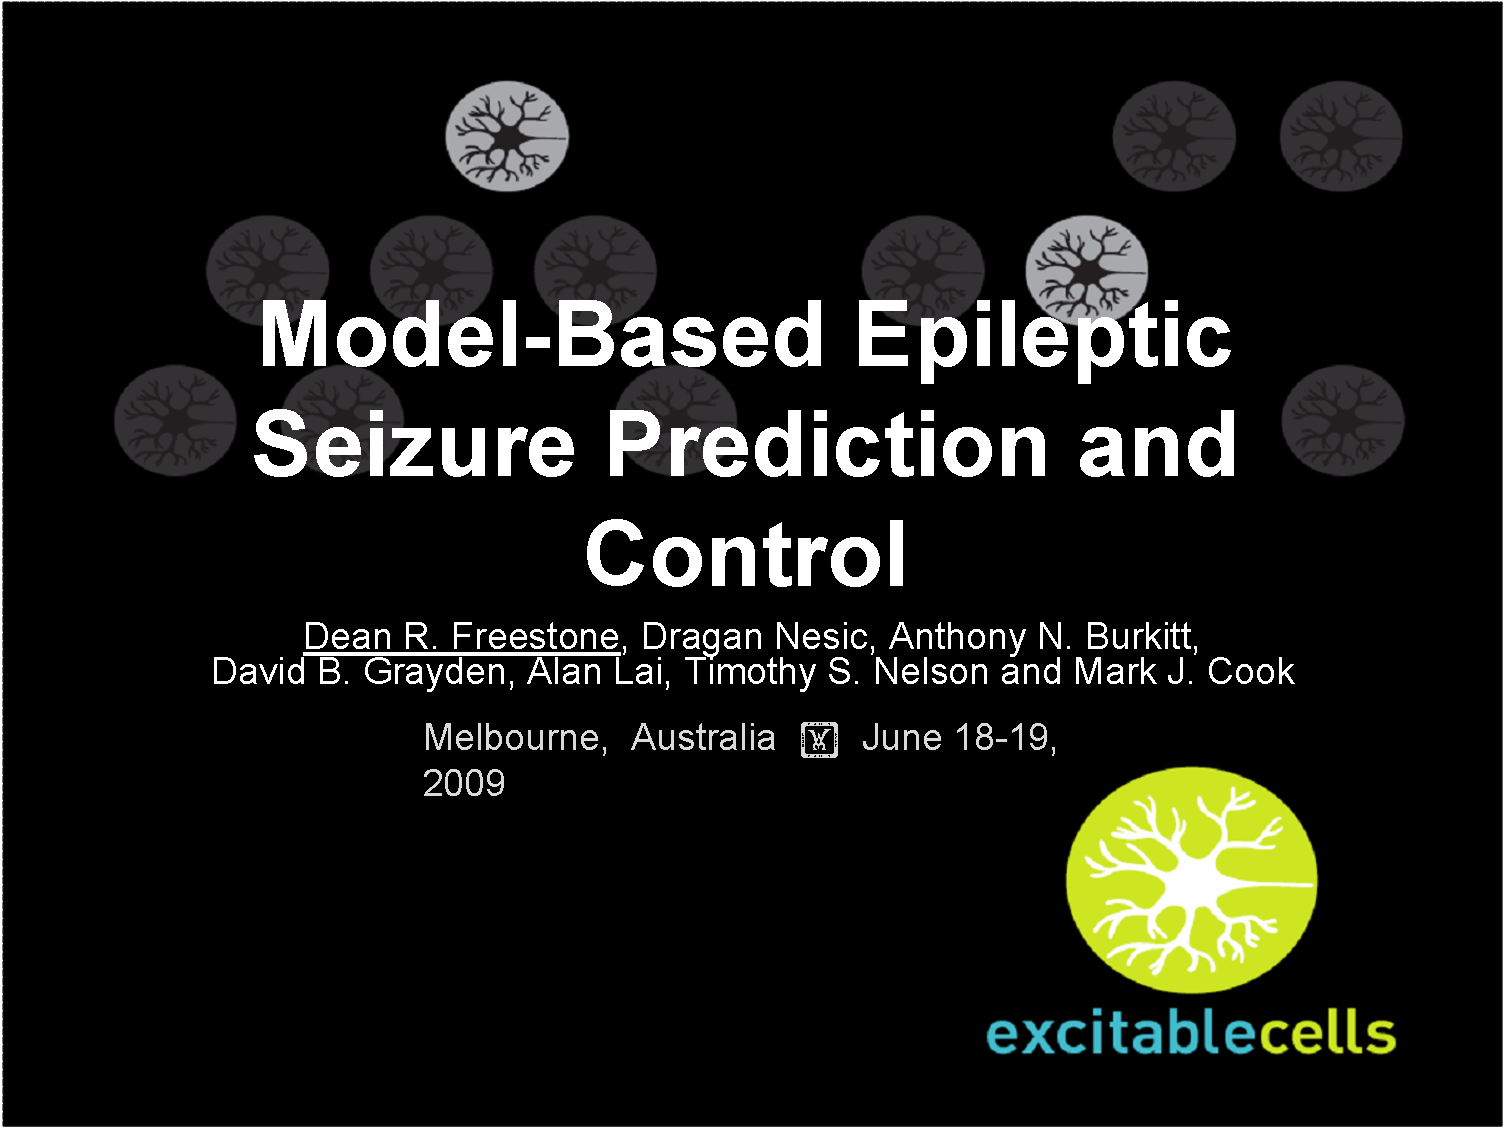
\includegraphics[height=5cm]{./Figures/SparkTitle.pdf}	
	\end{center}	
\end{frame}

\begin{frame}
	\begin{center}
		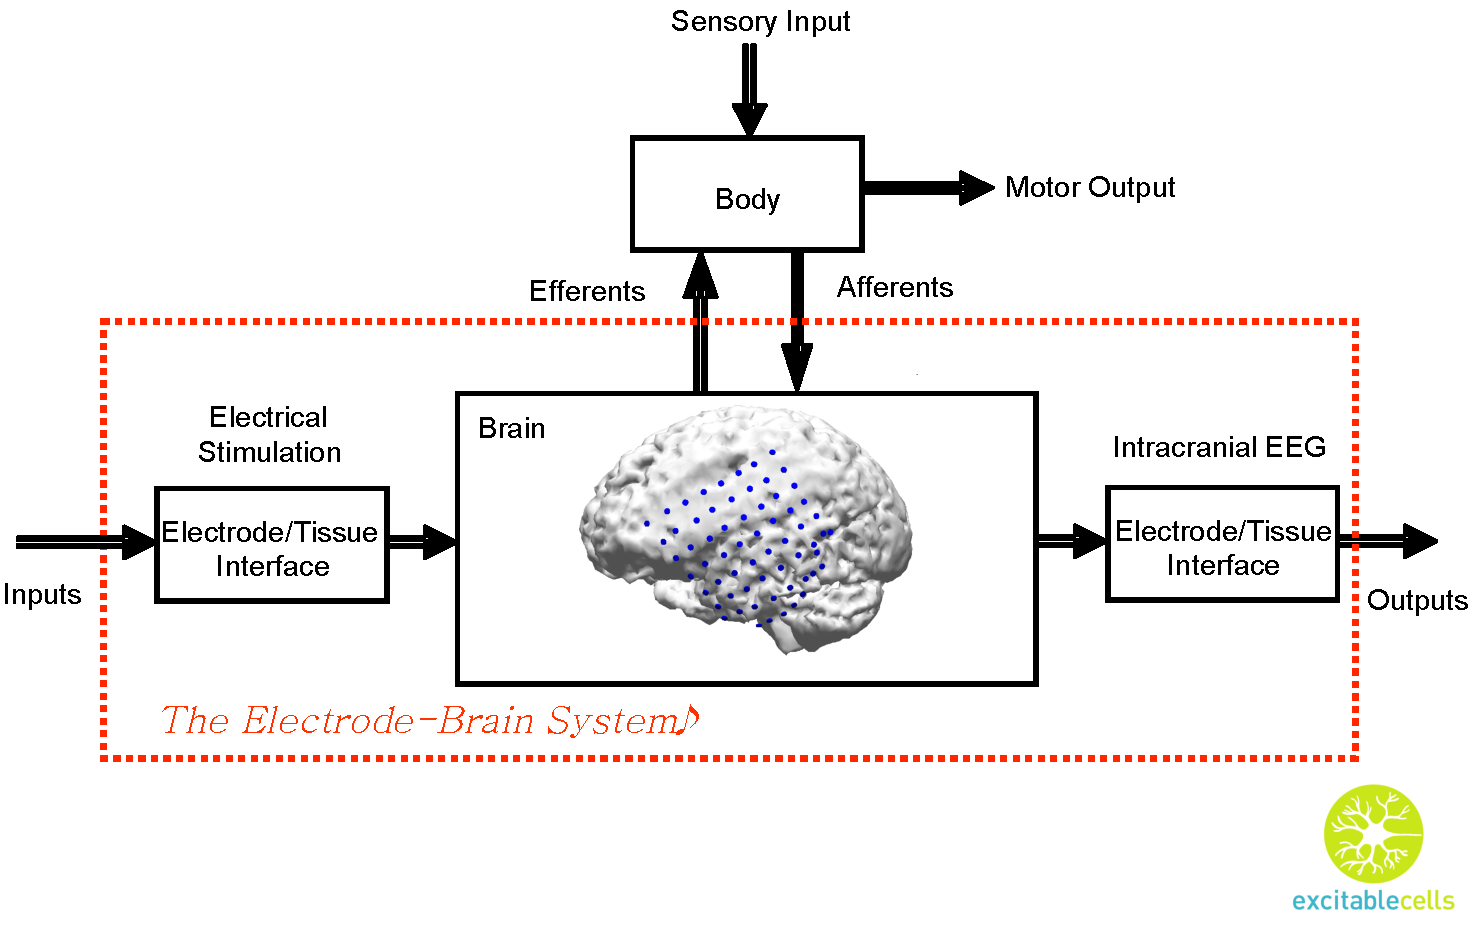
\includegraphics[height=5cm]{./Figures/BodyBrainElectrodeSystem.pdf}	
	\end{center}	
\end{frame}

\begin{frame}
	\begin{center}
		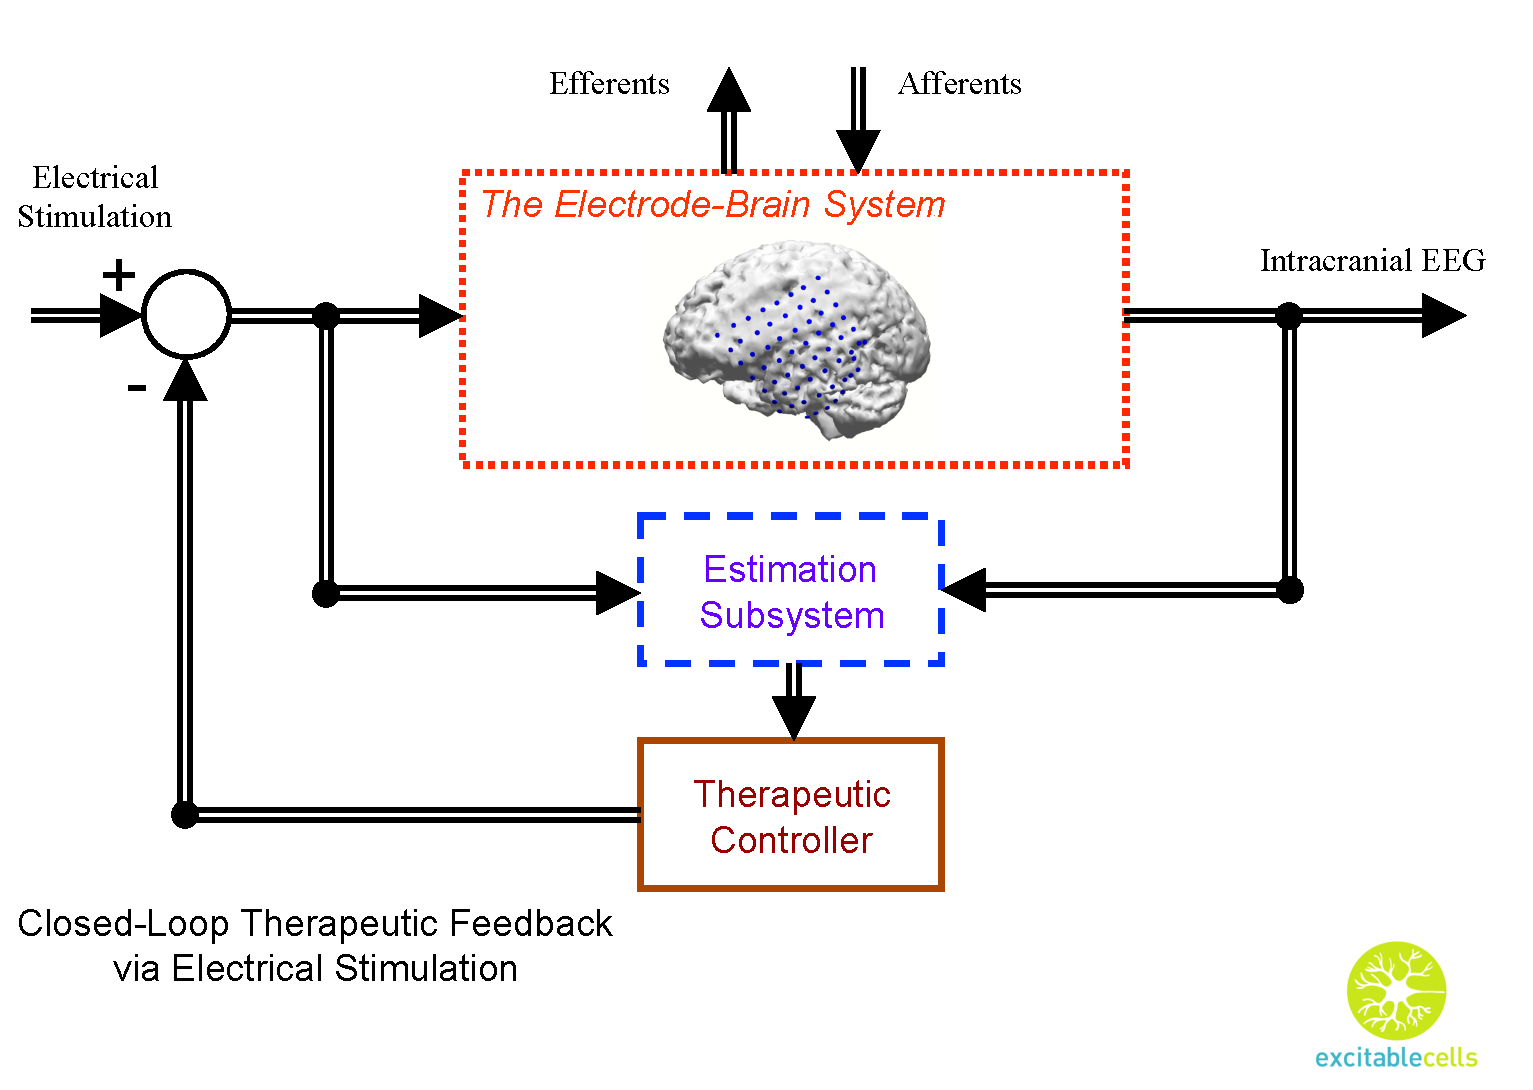
\includegraphics[height=5cm]{./Figures/StimulationSeizureControl.pdf}	
	\end{center}	
\end{frame}

\begin{frame}\frametitle{Patient specific model}
	Aim: To track the patient-specific neural dynamics and estimate the parameters that influence seizures from electrophysiological measurements. 
	\begin{center}
		\includegraphics<1>[height=6cm]{./Figures/BrainElectrode.pdf} 
	\end{center}
\end{frame}

\begin{frame}\frametitle{Measurement Modalities - Resected Tissue}
	% Aim: To track the patient-specific neural dynamics and estimate the parameters that influence seizures from electrophysiological measurements. 
	\begin{center}
		\includegraphics<1>[height=6cm]{./Figures/spatiotemporalscales.pdf} 
	\end{center}
\end{frame}

\begin{frame}\frametitle{Modelling approaches} 
	\begin{center}
		\includegraphics<1>[height=3cm]{./Figures/ModellingApproaches.pdf} 
	\end{center}
\end{frame}
\subsection{Fitting neural models to EEG}

% \begin{frame} \frametitle{Previous studies}
% \begin{itemize}
% 	\item Valdes et al. (1999) - local linearisation filter (Ozaki) with neural mass of Lopes Da Silva.
% 	\item David and Friston (2003) - Bayesian-based DCM framework, using coupled neural masses of Jansen and Rit.
% 	\item Galka et al. (2008) - Linear damped wave equation.
% 	\item Daunizeau et al. (2009) - DCM framework extended to neural fields.
% 	\item Schiff et al. (2008) - Used UKF with modified Wilson and Cowan equation.
% \end{itemize}
% \end{frame}

\section[Methodology]{Methodology}

\subsection[Neural field model]{Neural field model}


\begin{frame}\frametitle{Neural mass}
	\begin{center}
		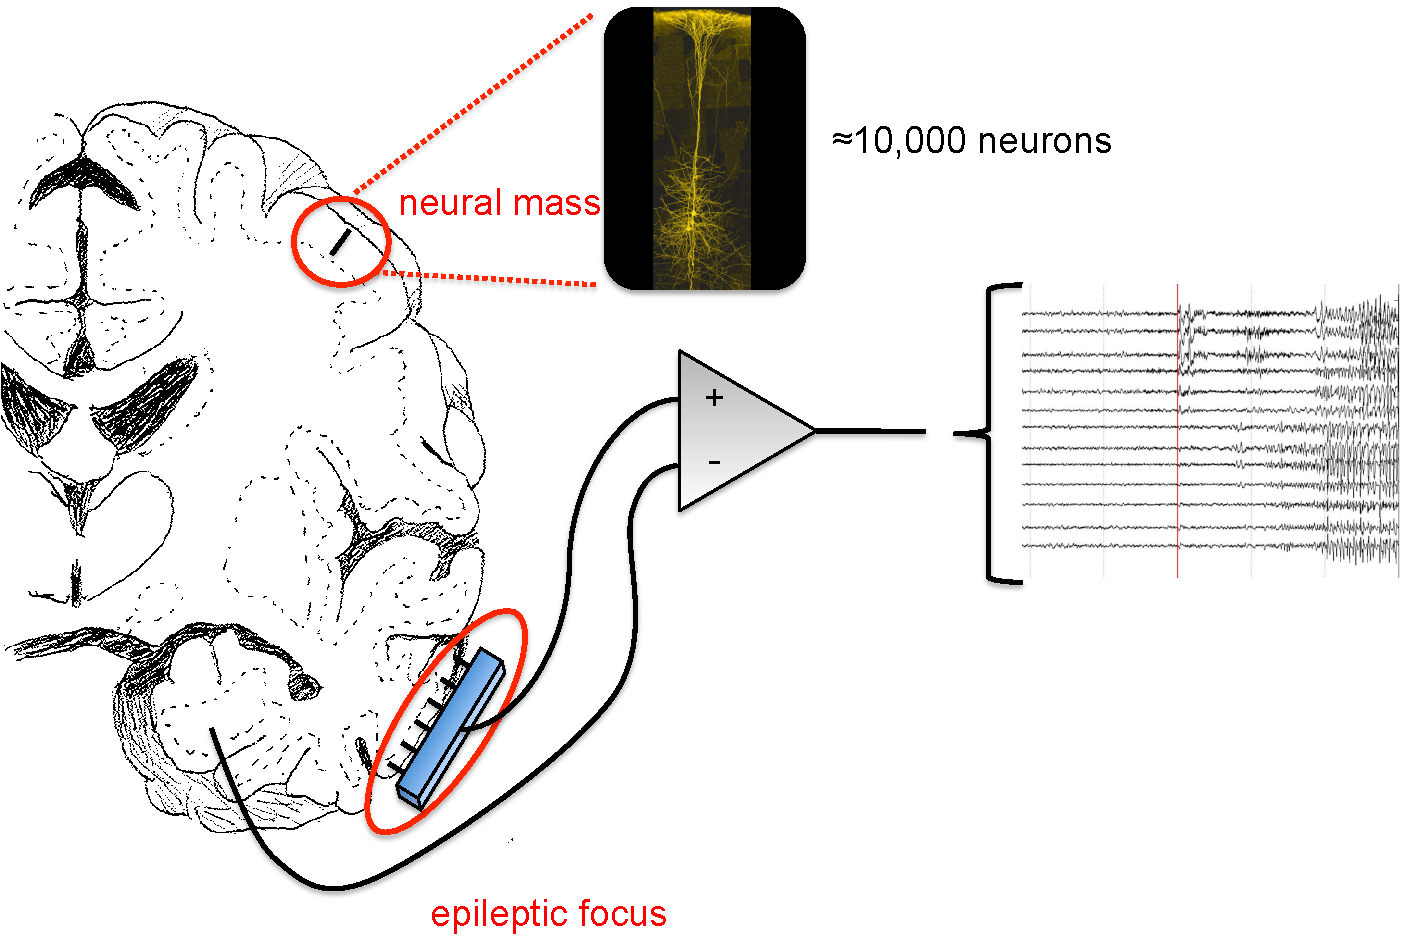
\includegraphics[height=6.5cm]{./Figures/NeuralMassWithSystem.pdf} 
	\end{center}
\begin{picture}(0,0)
	\put(-20,-40){\tiny Photo: Ecole Polytechnique Federale de Lausanne, HPC photo gallery, \emph{Golden Pyramids in Columns}}
\end{picture}
\end{frame}

\begin{frame}\frametitle{Neural mass}
	\begin{center}
		\includegraphics<1>[height=5cm]{./Figures/NeuralMass1.pdf} 
	\end{center}
\begin{picture}(0,0)
	\put(-20,-40){\tiny Photo: Ecole Polytechnique Federale de Lausanne, HPC photo gallery, \emph{Golden Pyramids in Columns}}
\end{picture}
\end{frame}

\begin{frame}\frametitle{Neural mass}
	\begin{center}
		\includegraphics<1>[height=5cm]{./Figures/NeuralMass2.pdf} 
\end{center}
\begin{align}
	g\left( \mathbf{r},t \right) &= {\color{orange}w_{\mathbf{r},\mathbf{r}'}}{\color{blue}f\left( v\left( \mathbf{r}',t \right) \right)} \\ 
	\color{blue}f\left( v\left( \mathbf{r}', t \right) \right) &= \frac{1}{1 + \exp \left( \varsigma \left( v_0 - v\left(\mathbf{r}',t\right) \right) \right)} 
\end{align}
\end{frame}


\begin{frame}\frametitle{Neural mass}
\begin{center}
	\includegraphics<1>[height=5cm]{./Figures/NeuralMass3.pdf} 
\end{center}
\begin{equation}
	\label{SynapticRespKernel} {\color{purple}h(t)} = \eta(t)\exp{\left(-\frac{t}{\tau}\right)} 
\end{equation}
\end{frame}


\begin{frame}\frametitle{Neural mass}
	\begin{center}
		\includegraphics<1>[height=5cm]{./Figures/NeuralMass4.pdf} 
	\end{center}
	\begin{equation}
		\label{SpikesToPotential} {\color{red} \underbrace{v\left( {\mathbf{r},t} \right) }_{\text{potential}}} = \int_{ - \infty }^t { {\color{purple}\underbrace{h\left( {t - t'} \right)}_{\text{synaptic}}} {\color{orange}\overbrace{w_{\mathbf{r},\mathbf{r}'}}^{\text{weight}}} {\color{blue}\underbrace{f\left( v\left( \mathbf{r}',t \right) \right)}_{\text{firing}}} \, dt'} 
	\end{equation}
\end{frame}

\begin{frame}\frametitle{Neural field}
	\begin{center}
		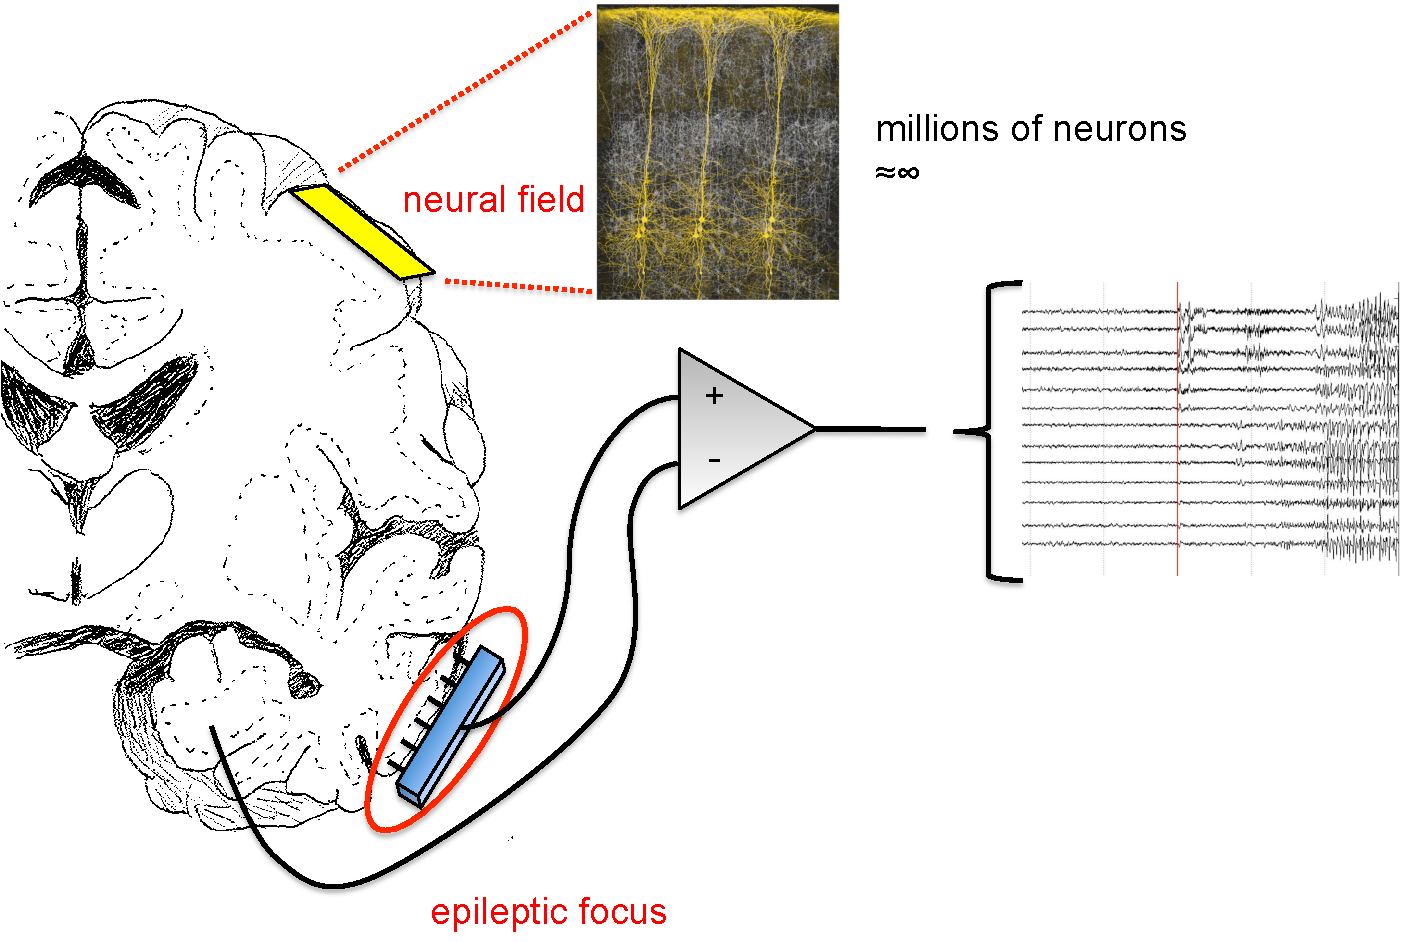
\includegraphics[height=6.5cm]{./Figures/NeuralFieldWithSystem.pdf} 
	\end{center}
\begin{picture}(0,0)
	\put(-20,-40){\tiny Photo: Ecole Polytechnique Federale de Lausanne, HPC photo gallery, \emph{Golden Pyramids in Columns}}
\end{picture}
\end{frame}

\begin{frame}\frametitle{Neural field model}
	\includegraphics<1->[height=4.5cm]{./Figures/Columns.pdf}
\begin{picture}(0,0)
	\put(-130,-115){\tiny Photo: Ecole Polytechnique Federale de Lausanne, HPC photo gallery, \emph{Golden Pyramids in Columns}}
\end{picture}
	\includegraphics<2->[height=.5cm]{./Figures/WhiteSpace.pdf}
	\includegraphics<2->[height=4.5cm]{./Figures/Anatomy.pdf}

\pause
\begin{equation}
	{\color{red} \underbrace{v\left( {\mathbf{r},t} \right) }_{\text{potential}}} = \int_{ - \infty }^t { {\color{purple}\underbrace{h\left( {t - t'} \right)}_{\text{synaptic}}} {\color{orange}\int_{\Omega}\overbrace{w\left(\mathbf{r},\mathbf{r}'\right)}^{\text{connectivity}}} {\color{blue}\underbrace{f\left( v\left( \mathbf{r}',t \right) \right)}_{\text{firing}}}\,\mathrm{d}\mathbf{r}' \, \mathrm{d}t'} 
\end{equation}

\pause
\begin{equation}
	{\color{darkgreen}\frac{\mathrm{d}v\left( \mathbf{r},t \right)}{\mathrm{d}t}} = {\color{purple}-\frac{1}{\tau} v\left( \mathbf{r},t \right)} +\int_{\Omega} {{\color{orange}w\left( \mathbf{r},\mathbf{r}' \right)}{\color{blue}f\left( {v\left( \mathbf{r}',t \right)} \right)}\, \mathrm{d}\mathbf{r}'}
\end{equation}
\end{frame}

\begin{frame}\frametitle{Discrete time stochastic neural field model}
	\begin{equation}
		\label{DiscreteTimeModel} 
		{\color{darkgreen}\underbrace{v_{t+T_s}\left(\mathbf{r}\right)}_{\text{dynamics}}} = 
		{\color{purple}\underbrace{\xi v_t\left(\mathbf{r}\right)}_{\text{synaptic}}} + 
		T_s \int_{\Omega} { 
		    {\color{orange}\underbrace{ w\left(\mathbf{r},\mathbf{r}'\right) }_{\text{connectivity}}}
		    {\color{blue}\underbrace{f\left(v_t\left(\mathbf{r}'\right)\right)}_{\text{firing}}} 
		\, d\mathbf{r}'} 
		+ {\color{brown}\underbrace{e_t\left(\mathbf{r}\right)}_{\text{uncertainty}}}, 
	\end{equation}
	where 
\begin{align}
	\xi &= 1-\frac{T_s}{\tau} \nonumber \\
	\color{brown}e_t(\mathbf{r})&\sim\mathcal{GP}(\mathbf 0,\gamma(\mathbf{r}-\mathbf{r}')) \nonumber
\end{align}
\begin{center}
	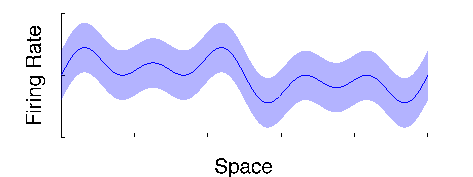
\includegraphics[height=3cm]{./Figures/FieldWithUncertainy.pdf} 
\end{center}
\end{frame}

\begin{frame}\frametitle{Observations}
	\begin{center}
		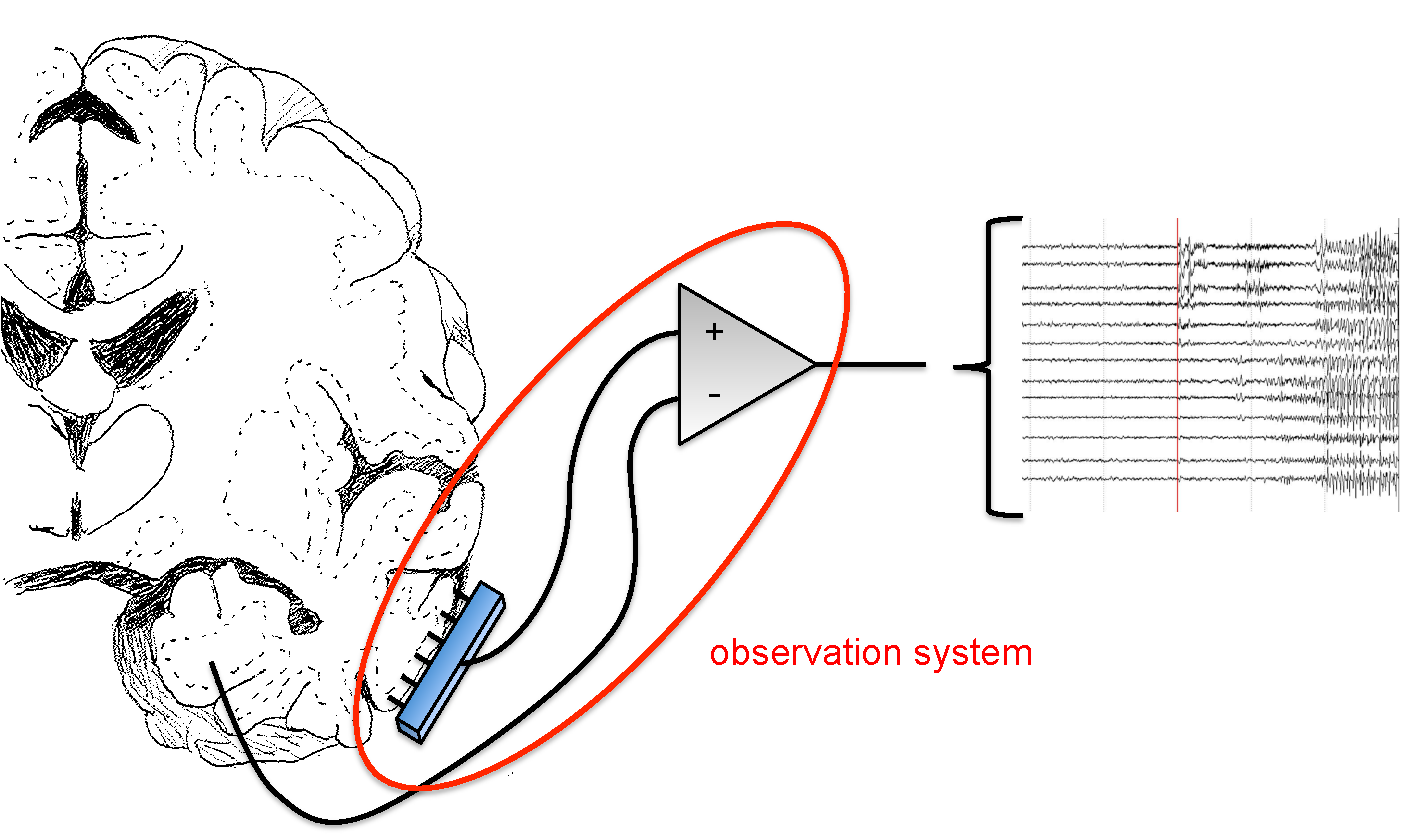
\includegraphics[height=6.5cm]{./Figures/ObservationSystem.pdf} 
	\end{center}
\begin{picture}(0,0)
	\put(-20,-40){\tiny Photo: Ecole Polytechnique Federale de Lausanne, HPC photo gallery, \emph{Golden Pyramids in Columns}}
\end{picture}
\end{frame}

\begin{frame}\frametitle{Observation equation}
	\includegraphics<1-2>[height=3.8cm]{./Figures/fig13.pdf}
	\includegraphics<2-2>[height=2cm]{./Figures/WhiteSpace.pdf}
	\includegraphics<2-2>[height=3.8cm]{./Figures/fig14.pdf}
	\begin{equation}\label{eq:ObservationEquation}
		\underbrace{y_t(\mathbf{r}_n)}_{\text{observation}} = \int_{\Omega} { {\color{cyan}\underbrace{m\left(\mathbf{r}_n-\mathbf{r}'\right)}_{\text{sensor}}} {\color{red}\underbrace{v_t\left(\mathbf{r}'\right)}_{\text{potential}}} \, d\mathbf{r}'} + {\color{magenta}\underbrace{\varepsilon_t(\mathbf{r}_n)}_{\text{noise}}}, 
	\end{equation}
	where
	\begin{align}
		\color{cyan} m\left(\mathbf{r}-\mathbf{r}'\right) &= \exp{\left(-\frac{(\mathbf{r}-\mathbf{r}')^\top(\mathbf{r}-\mathbf{r}')}{\sigma_m^2}\right)} \\
		\color{magenta}\varepsilon_t(\mathbf{r}_n) &\sim \mathcal{N}\left(0,\boldsymbol{\Sigma}_{\varepsilon}\right).
	\end{align}
	\pause
	\includegraphics<3-5>[height=3.8cm]{./Figures/SensorKernel1.pdf}
	\includegraphics<4-5>[height=3.8cm]{./Figures/SensorKernel2.pdf}
	\includegraphics<5-5>[height=3.8cm]{./Figures/SensorKernel3.pdf}
\end{frame}

\begin{frame}\frametitle{Spatial aliasing}
	\includegraphics<1-2>[height=6cm]{./Figures/205px-Moire_pattern_of_bricks.pdf}
	\includegraphics<2>[height=0.5cm]{./Figures/WhiteSpace.pdf}
	\includegraphics<2>[height=6cm]{./Figures/Moire_pattern_of_bricks_small.pdf}	
\end{frame}

\begin{frame}\frametitle{Positioning sensors}
Assuming
\begin{equation}
	V_t(\boldsymbol{\nu}) \approx 0 ~ \ \forall \boldsymbol{\nu} > \boldsymbol{\nu}_c,
\end{equation}
where $\boldsymbol\nu$ is the spatial frequency. 
\begin{center}
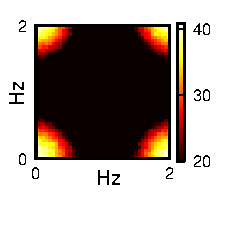
\includegraphics[height=3.5cm]{./Figures/Figure4a.pdf}
\end{center}
\pause
\begin{equation}
	\label{eq:MinimumSensorDistance} \Delta_y \leq \frac{1}{2\rho_y\boldsymbol{\nu}_{c}}, 
\end{equation}
where $\rho_y \in \mathbb{R} \ge 1$. See Scerri et al. for more info\footnote{Scerri et al. (2009) IEEE Trans. Sig. Proc. 57}. \\ 
\end{frame}

\begin{frame}\frametitle{Field spatial frequency}
	\begin{itemize}
\item Freeman\footnote{Freeman et al. (2000) J. Neurosci. Meth. 95.} estimated $\boldsymbol{\nu}_c$ to be approximately 0.25~cycles/mm.
\pause
  \item This implies $\Delta_y \lesssim 1.25$ mm to prevent aliasing.
\pause
  \item Electrodes satisfying this requirement are in clinical use.
 \end{itemize}
	\begin{center}
		\includegraphics[height=5cm]{./Figures/UtahArray.pdf}
	\end{center}
\end{frame}


\begin{frame}\frametitle{Model output}
	\begin{align}
		{\color{darkgreen}v_{t+T_s}\left(\mathbf{r}\right)} &= 
		{\color{purple}\xi v_t\left(\mathbf{r}\right)} + 
		T_s \int_\Omega { 
		    {\color{orange}w\left(\mathbf{r},\mathbf{r}'\right)}
		    {\color{blue}f\left(v_t\left(\mathbf{r}'\right)\right)} 
		\, d\mathbf{r}'} 
		+ {\color{brown}e_t\left(\mathbf{r}\right)} \nonumber \\
		y_t(\mathbf{r}_n) &= \int_{\Omega} { {\color{cyan}m\left(\mathbf{r}_n-\mathbf{r}'\right)} {\color{red}v_t\left(\mathbf{r}'\right)} \, d\mathbf{r}'} + {\color{magenta}\varepsilon_t(\mathbf{r}_n)} \nonumber 
	\end{align}
\begin{center} 
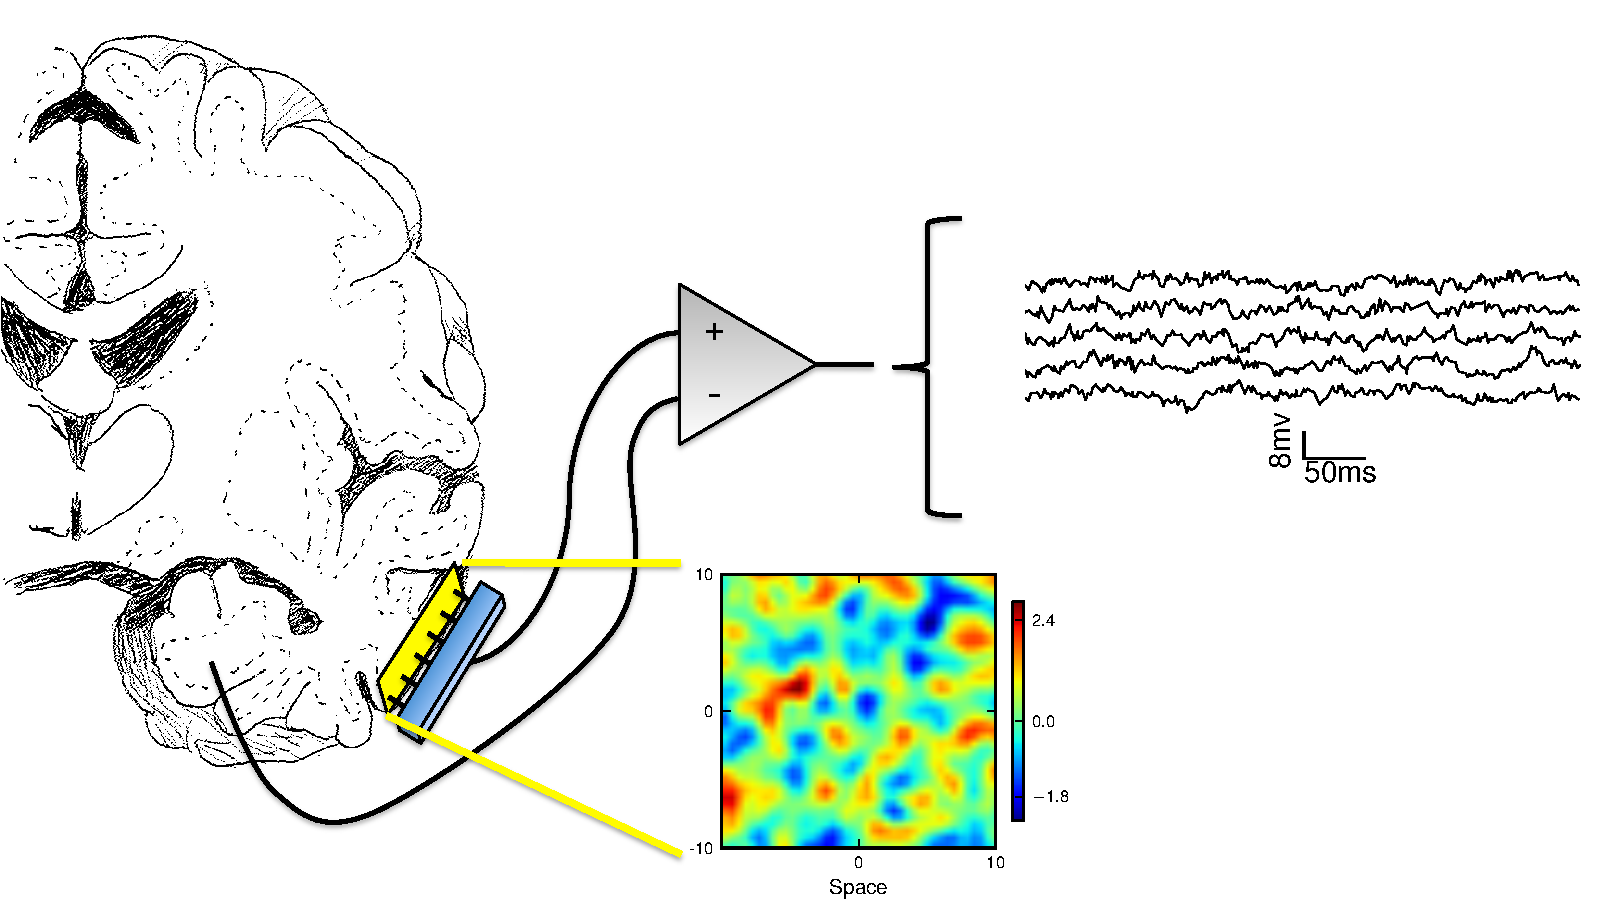
\includegraphics[height=6cm]{./Figures/ModelOutput.pdf}
\end{center}
\end{frame}

%%%%%%%%%%%%%%%%%%%%%%%%%


\begin{frame}\frametitle{Aim again}
Aim: To track the patient-specific neural dynamics and estimate the parameters that influence seizures from electrophysiological measurements.
\begin{align}
	{\color{darkgreen} \underbrace{v_{t+T_s}\left(\mathbf{r}\right)}_{\text{dynamics}}} &= 
	{\color{purple}\underbrace{\xi v_t\left(\mathbf{r}\right)}_{\text{synaptic}}} + 
	T_s \int_\Omega { 
	    {\color{orange}\underbrace{w\left(\mathbf{r},\mathbf{r}'\right)}_{\text{connectivity}}}
	    {\color{blue}\underbrace{f\left(v_t\left(\mathbf{r}'\right)\right)}_{\text{firing}}} 
	\, d\mathbf{r}'} 
	+ {\color{brown}\underbrace{e_t\left(\mathbf{r}\right)}_{\text{uncertainty}}} \nonumber \\
	\underbrace{y_t(\mathbf{r}_n)}_{\text{observation}} &= \int_{\Omega} { {\color{cyan}\underbrace{m\left(\mathbf{r}_n-\mathbf{r}'\right)}_{\text{sensor}}} {\color{red}\underbrace{v_t\left(\mathbf{r}'\right)}_{\text{potential}}} \, d\mathbf{r}'} + {\color{magenta}\underbrace{\varepsilon_t(\mathbf{r}_n)}_{\text{noise}}} \nonumber 
\end{align}
\end{frame}

\subsection[Kernel basis function decomposition]{Kernel basis function decomposition}

\begin{frame} \frametitle{Connectivity kernel decomposition}
\begin{equation}\label{DefKernelDecomp}
	 {\color{orange}w\left(\mathbf{r},\mathbf{r}'\right)} = {\color{orange}\boldsymbol{\psi}^\top\left(\mathbf{r},\mathbf{r}'\right) \boldsymbol{\theta}}
\end{equation}
\begin{center}
\includegraphics<1>[height=3.8cm]{./Figures/Kernel1.pdf}
\end{center}
\includegraphics<2>[height=3.8cm]{./Figures/Kernel2.pdf}
\includegraphics<2>[height=3.8cm]{./Figures/Kernel3.pdf}
\includegraphics<2>[height=3.8cm]{./Figures/Kernel4.pdf}
\begin{center}
\includegraphics<3>[height=3.8cm]{./Figures/fig1.pdf}
\end{center}
\end{frame}

\begin{frame}\frametitle{Aim again, again}
Aim: To track the patient-specific neural dynamics and estimate the parameters that influence seizures from electrophysiological measurements.	
	\begin{align}
		{\color{darkgreen}v_{t+T_s}\left(\mathbf{r}\right)} &= 
		{\color{purple}\xi v_t\left(\mathbf{r}\right)} + 
		T_s \int_\Omega { 
		    {\color{blue}f\left(v_t\left(\mathbf{r}'\right)\right)} 
			{\color{orange}\boldsymbol\psi^{\top}\left(\mathbf{r},\mathbf{r}'\right)}
		\, d\mathbf{r}'} {\color{orange}\boldsymbol\theta}
		+ {\color{brown}e_t\left(\mathbf{r}\right)} \nonumber \\
		y_t(\mathbf{r}_n) &= \int_{\Omega} { {\color{cyan}m\left(\mathbf{r}_n-\mathbf{r}'\right)} {\color{red}v_t\left(\mathbf{r}'\right)} \, d\mathbf{r}'} + {\color{magenta}\varepsilon_t(\mathbf{r}_n)} \nonumber 
	\end{align}	
\end{frame}

\subsection[Field basis function decomposition]{Field basis function decomposition}

\begin{frame}\frametitle{Field basis function decomposition}
We can approximate the field by
\begin{equation}
		\label{DefFieldDecomp} {\color{red}v_t\left(\mathbf{r}\right)} \approx {\color{red}\boldsymbol{\phi}^{\top}\left(\mathbf{r}\right) \mathbf{x}_t},
\end{equation}
where
$$ \phi\left(\mathbf{r}-\mathbf{r}'\right) =
\exp{\left(-\frac{(\mathbf{r}-\mathbf{r}')^\top(\mathbf{r}-\mathbf{r}')}{\sigma_{\phi}^2}\right)}. $$
\end{frame}

% \begin{frame} \frametitle{1D neural field}
% \begin{center}	
% \frame{\movie[height=188pt,width=242pt,poster,autoplay,repeat]{}{./Figures/1DFieldDemo.mov}}
% \end{center}
% \end{frame}
% 
% \begin{frame} \frametitle{1D neural field decomposition}
% \begin{center}	
% \frame{\movie[height=188pt,width=242pt,poster,autoplay,repeat]{}{./Figures/1DFieldWithBasisFunctionDemo.mov}}
% \end{center}
% \end{frame}

\begin{frame} \frametitle{1D neural field decomposition with state}
	A movie was here
% \begin{center}	
% \frame{\movie[height=188pt,width=242pt,poster,autoplay,repeat]{}{./Figures/1DFieldDemoWithBasisFunctionAndState.mov}}
% \end{center}
\end{frame}

\begin{frame}\frametitle{Sensor and field basis function position}
	\begin{center}
		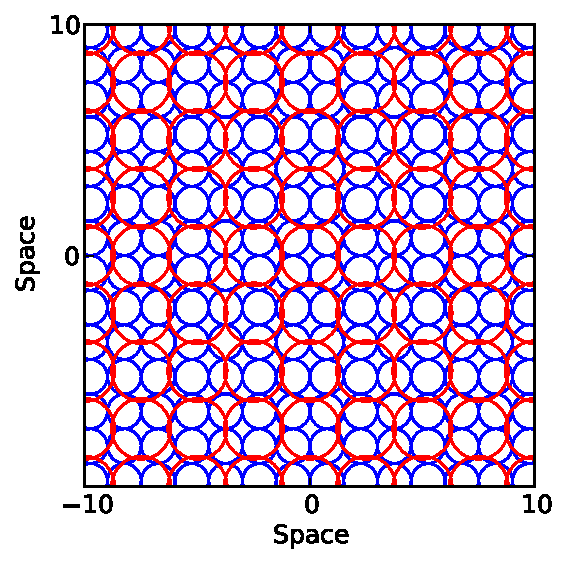
\includegraphics[height=7cm]{./Figures/FieldAndSensors.pdf}
	\end{center}
\end{frame}

\begin{frame}\frametitle{Reduced system equation}
We get a reduced system equation
\begin{equation}
	{\color{darkgreen}\boldsymbol{\phi}^{\top}(\mathbf{r})\mathbf{x}_{t+T_s}} = 
	{\color{purple}\xi \boldsymbol{\phi}^{\top}(\mathbf{r})\mathbf{x}_{t}} + 
	T_s \int_\Omega { 
	    {\color{blue}f\left(\boldsymbol{\phi}^{\top}(\mathbf{r})\mathbf{x}_{t}\right)} 
		{\color{orange}\boldsymbol\psi^{\top}\left(\mathbf{r},\mathbf{r}'\right)}
	\, d\mathbf{r}'} {\color{orange}\boldsymbol\theta}
	+ {\color{brown}e_t\left(\mathbf{r}\right)}.
\end{equation}
\pause
This simplifies to
\begin{align}
	{\color{darkgreen}\mathbf{x}_{t+1}} = {\color{purple}\xi\mathbf{x}_t} 
+ \int_\Omega {\color{orange}\boldsymbol{\Psi}(\mathbf{r}')} {\color{blue}f(\boldsymbol{\phi}^{\top}(\mathbf{r}')\mathbf{x}_t)} \, d\mathbf{r}' {\color{orange}\boldsymbol{\theta}} + {\color{brown}\mathbf{e}_t},
\end{align}
\pause
where
\begin{align}
	\color{brown}\mathbf{e}_t &\triangleq \boldsymbol{\Gamma}^{-1}\int_\Omega {\boldsymbol{\phi} ( \mathbf{r} )e_t( \mathbf{r} ) \, d\mathbf{r}} \\
	\boldsymbol{\Gamma} &\triangleq \int_\Omega {\boldsymbol{\phi} \left(\mathbf{r}\right)\boldsymbol{\phi} ^{\top}\left(\mathbf{r}\right) \, d\mathbf{r}} \\
	\color{orange}\left[ \boldsymbol\Psi(\mathbf{r}')\right]_{:i}  &\triangleq T_s\boldsymbol{\Gamma}^{-1}\int_\Omega {\boldsymbol{\phi}(\mathbf{r})\psi_i (2\mathbf{c}_i+\mathbf{r}'-\mathbf{r})\textrm{d}\mathbf{r}}.
\end{align}
\end{frame}

\begin{frame}\frametitle{Reduced observation equation}
	\begin{equation}
		y_t(\mathbf{r}_n) = \int_{\Omega} { {\color{cyan}m\left(\mathbf{r}_n-\mathbf{r}'\right)} {\color{red}\boldsymbol{\phi}^{\top}(\mathbf{r})\mathbf{x}_{t}} \, d\mathbf{r}'} + {\color{magenta}\varepsilon_t(\mathbf{r}_n)} 
	\end{equation}
\pause
In the more compact form
\begin{equation}\label{ObservationEquation} 
	\mathbf{y}_t = {\color{cyan}\mathbf{C}}{\color{red}\mathbf{x}_t} + {\color{magenta}\boldsymbol{\varepsilon}_t},
\end{equation}
\pause
where each element of the observation matrix, $\mathbf{C}$, is 
\begin{equation}
	{\color{cyan}\mathbf{C}_{ij}} \triangleq \int_{\Omega}m(\mathbf{r}_i - \mathbf{r}')\boldsymbol{\phi}_j(\mathbf{r}') \, d\mathbf{r}'.
\end{equation}
\end{frame}
	
\begin{frame}\frametitle{Aim again, again, again}
Aim: To track the patient-specific neural dynamics and estimate the parameters that influence seizures from electrophysiological measurements.	
	\begin{align}
		{\color{darkgreen}\mathbf{x}_{t+1}} &= {\color{purple}\xi\mathbf{x}_t} 
	+ \int_\Omega {\color{orange}\boldsymbol{\Psi}(\mathbf{r}')} {\color{blue}f(\boldsymbol{\phi}^{\top}(\mathbf{r}')\mathbf{x}_t)} \, d\mathbf{r}' {\color{orange}\boldsymbol{\theta}} + {\color{brown}\mathbf{e}_t} \nonumber \\
	\mathbf{y}_t &= {\color{cyan}\mathbf{C}}\mathbf{x}_t + {\color{magenta}\boldsymbol{\varepsilon}_t}\nonumber 
	\end{align}
	\pause
	We need to estimate the states, $\mathbf{x}_t$, and parameters, $\boldsymbol\theta$ and $\xi$, given the prerecorded observations, $\mathbf{y}_t$.
\end{frame}


\subsection[Estimation algorithm]{Estimation algorithm}


\begin{frame}\frametitle{Estimation algorithm}
We need to estimate the states, $\mathbf{x}_t$, and parameters, $\boldsymbol\theta$ and $\xi$, given the prerecorded observations, $\mathbf{y}_t$. (see refs\footnote{Ljung, L., (1999); Haykin, S., (2001); Sarkka, S., (2010); Julier, S. and Uhlmann, J., (1997).})
\begin{center}
	\includegraphics<1>[height=4cm]{./Figures/EstimationAlgorithm1.pdf}
	\includegraphics<2>[height=4cm]{./Figures/EstimationAlgorithm2.pdf}
	\includegraphics<3>[height=4cm]{./Figures/EstimationAlgorithm3.pdf}
	\includegraphics<4>[height=4cm]{./Figures/EstimationAlgorithm4.pdf}
	% \includegraphics<5>[height=3cm]{./Figures/EstimationAlgorithm5.pdf}
	\includegraphics<5>[height=4cm]{./Figures/EstimationAlgorithm6.pdf}
	\includegraphics<6>[height=4cm]{./Figures/EstimationAlgorithm7.pdf}
	\includegraphics<7>[height=4cm]{./Figures/EstimationAlgorithm8.pdf}
\end{center}
\end{frame}

\begin{frame}\frametitle{Parameter estimation - least squares}
	Assume we have an estimate (guess) for $\hat{\mathbf{x}}_{t} = \hat{\mathbf{x}}_{0}, \hat{\mathbf{x}}_{1}, \hat{\mathbf{x}}_{2}, \hdots, \hat{\mathbf{x}}_{T}$ \pause and
	\begin{equation}
			{\color{darkgreen}\mathbf{x}_{t+1}} = {\color{purple}\xi\mathbf{x}_t} 
		+ \underbrace{\int_\Omega {\color{orange}\boldsymbol{\Psi}(\mathbf{r}')} {\color{blue}f(\boldsymbol{\phi}^{\top}(\mathbf{r}')\mathbf{x}_t)} \, d\mathbf{r}' }_{\mathbf{q}(\hat{\mathbf{x}}_t)}{\color{orange}\boldsymbol{\theta}} + {\color{brown}\mathbf{e}_t}.
	\end{equation}
\pause
Given the estimated state sequence we can write
\begin{align*}
	 \hat{\mathbf x}_{1} &= \mathbf{q}(\hat{\mathbf x}_0) \boldsymbol{\theta}+\xi\hat{\mathbf x}_0+\mathbf e_0 \\
	\hat{\mathbf x}_{2} &= \mathbf{q}(\hat{\mathbf x}_1) \boldsymbol{\theta}+\xi\hat{\mathbf x}_1+\mathbf e_1  \\
	&\vdots& \\
	\hat{\mathbf x}_{T}&= \mathbf{q}(\hat{\mathbf x}_{T-1}) \boldsymbol{\theta}+\xi\hat{\mathbf x}_{T-1}+\mathbf e_{T-1}. 
\end{align*}
\pause
This can be written in the compact form
\begin{equation}
	\mathbf Z=\mathbf X \mathcal W+\mathbf{e}, 
\end{equation}
\end{frame}

\begin{frame}\frametitle{Parameter estimation continued}
\begin{equation}
	\mathbf Z=\mathbf X \mathcal W+\mathbf{e}, 
\end{equation}
\pause
where
\begin{small}
\begin{equation*}
	\mathbf Z=\left[
	\begin{array}{cccc}
		\hat{\mathbf x}_{1}\\
		\hat{\mathbf x}_{2}\\
		\vdots\\
		\hat{\mathbf x}_{T}
	\end{array}
	\right],\quad \mathbf X=\left[
	\begin{array}{cccc}
		\mathbf q(\hat{\mathbf x}_0)& \hat{\mathbf x}_{0}\\
		\mathbf q(\hat{\mathbf x}_1)& \hat{\mathbf x}_{1}\\
		\vdots & \vdots\\
		\mathbf q(\hat{\mathbf x}_{T-1})& \hat{\mathbf x}_{T-1}
	\end{array}
	\right] 
\end{equation*}
\end{small}
and
\begin{small}
\begin{equation*}
\quad \mathcal W=\left[
	\begin{array}{cc}
		\boldsymbol{\theta} \\
		\xi
	\end{array}
	\right],\quad \mathbf{e}=\left[
	\begin{array}{cccc}
		\mathbf e_0\\
		\mathbf e_1\\
		\vdots\\
		\mathbf e_{T-1}
	\end{array}
	\right].
\end{equation*}
\end{small}
\pause
The closed-form solution is
\begin{equation}
	\hat{\mathcal{W}}=(\mathbf X^\top\mathbf X)^{-1}\mathbf X^\top\mathbf Z. 
\end{equation}
\end{frame}

\begin{frame}\frametitle{Idea of Kalman Filter}
\begin{center}
	\includegraphics<1>[height=8cm,angle=90]{./Figures/KalmanSketch1.pdf}
	\includegraphics<2>[height=8cm,angle=90]{./Figures/KalmanSketch2.pdf}
	\includegraphics<3>[height=8cm,angle=90]{./Figures/KalmanSketch3.pdf}
	\includegraphics<4>[height=8cm,angle=90]{./Figures/KalmanSketch4.pdf}
\end{center}
\end{frame}

\begin{frame}\frametitle{Estimation algorithm}
\begin{center}
	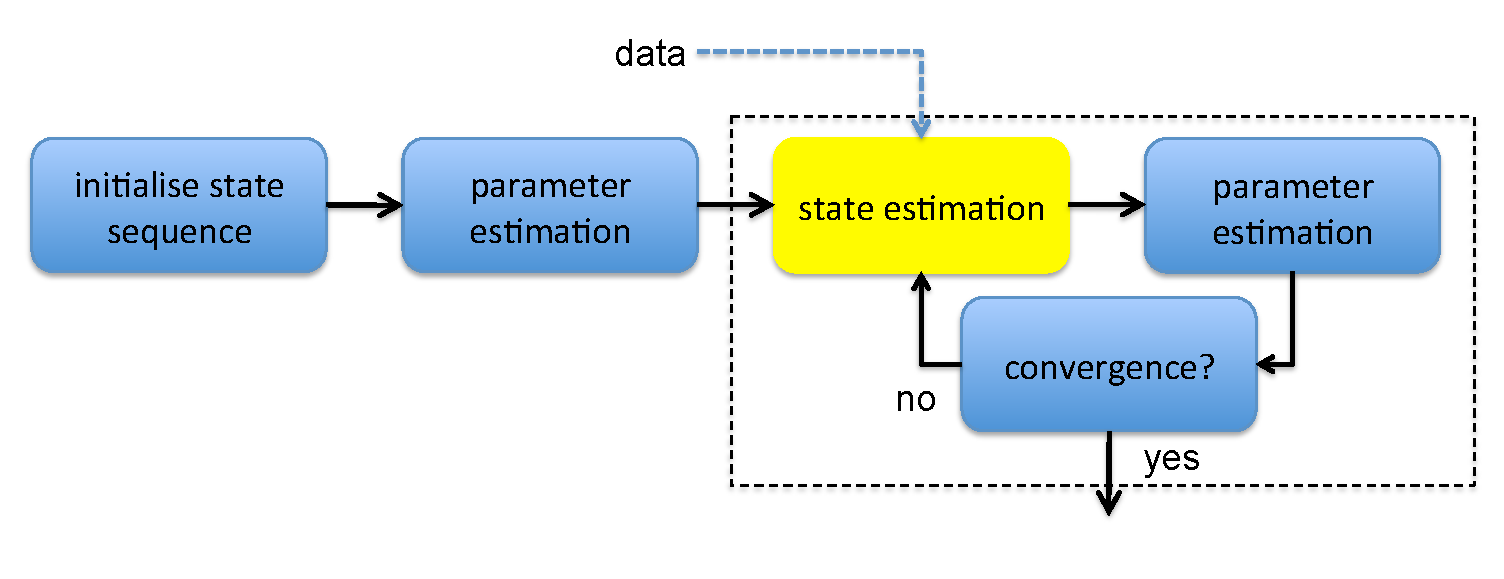
\includegraphics[height=4cm]{./Figures/EstimationAlgorithm9.pdf}
\end{center}
\end{frame}

\begin{frame}\frametitle{State estimation - Kalman filter}
	\includegraphics<1>[height=6cm]{./Figures/KalmanFilter1.pdf}
	\includegraphics<2>[height=6cm]{./Figures/KalmanFilter2.pdf}
	\includegraphics<3>[height=6cm]{./Figures/KalmanFilter3.pdf}
	\includegraphics<4>[height=6cm]{./Figures/KalmanFilter4.pdf}
	\includegraphics<5>[height=6cm]{./Figures/KalmanFilter5.pdf}
	\includegraphics<6>[height=6cm]{./Figures/KalmanFilter6.pdf}
	\includegraphics<7>[height=6cm]{./Figures/KalmanFilter7.pdf}
	\includegraphics<8>[height=6cm]{./Figures/KalmanFilter8.pdf}
	\includegraphics<9>[height=6cm]{./Figures/KalmanFilter9.pdf}
	\includegraphics<10>[height=6cm]{./Figures/KalmanFilter10.pdf}
	\includegraphics<11>[height=6cm]{./Figures/KalmanFilter11.pdf}
	\includegraphics<12>[height=6cm]{./Figures/KalmanFilter12.pdf}
\end{frame}

\begin{frame}\frametitle{Estimation algorithm}
\begin{center}
	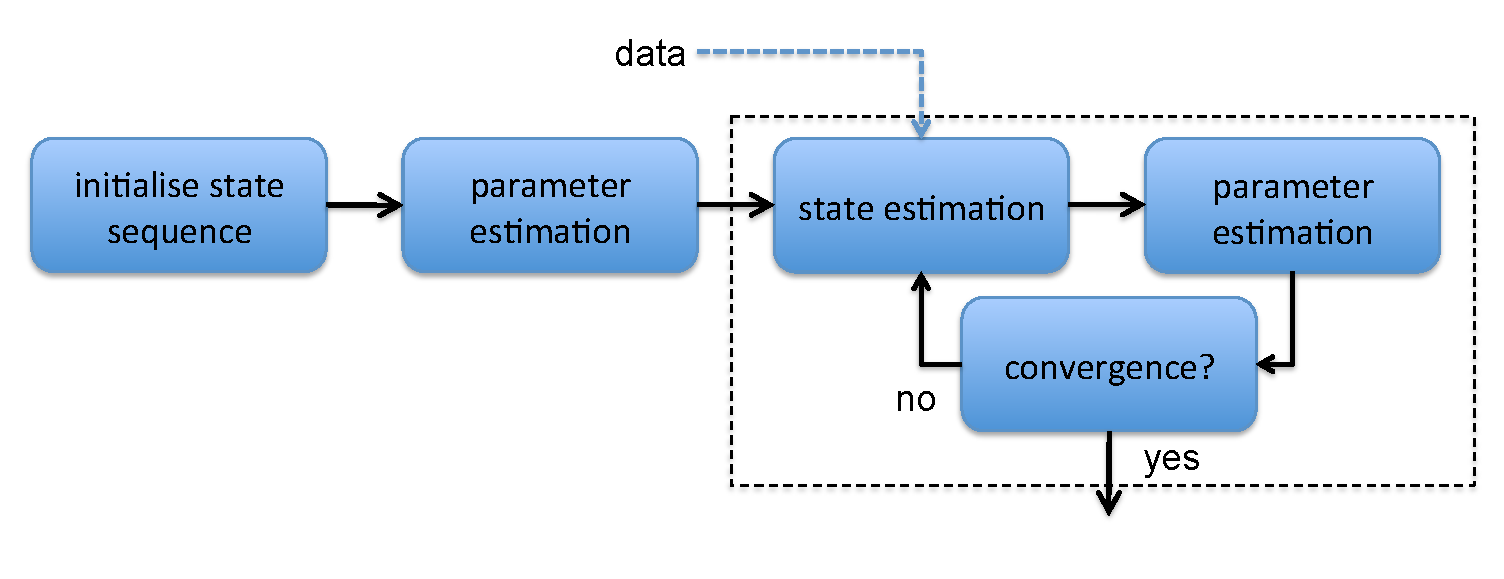
\includegraphics[height=4cm]{./Figures/EstimationAlgorithm7.pdf}
\end{center}
\end{frame}

\section[Results]{Results}

\begin{frame}\frametitle{Experimental setup}
\begin{itemize}
	\item 150 realisations of data using model (Monte Carlo)
	\item Set the model parameters to be realistic
	\item Use the data-driven framework to perform state and parameters estimation
	\item Compare estimated parameters to actual parameters
	\item Compare the estimated neural field to actual field
\end{itemize}	
\end{frame}

\begin{frame}\frametitle{Monte Carlo simulation results - convergence}
	\begin{center}
		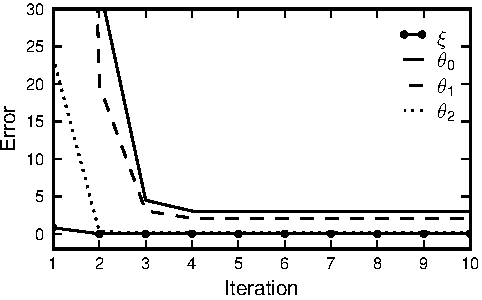
\includegraphics[height=6cm]{./Figures/fig6.pdf}
	\end{center}
\end{frame}

\begin{frame}\frametitle{Monte Carlo simulation results - distributions}
	\begin{center}
		\includegraphics<1>[height=2.5cm]{./Figures/Figure7a.pdf}
		\includegraphics<1>[height=2.5cm]{./Figures/Figure7b.pdf}
		\includegraphics<1>[height=2.5cm]{./Figures/Figure7c.pdf}
		\includegraphics<1>[height=2.5cm]{./Figures/Figure7d.pdf}\\
		\includegraphics<1>[height=2.5cm]{./Figures/Kernel2.pdf}
		\includegraphics<1>[height=2.5cm]{./Figures/Kernel3.pdf}
		\includegraphics<1>[height=2.5cm]{./Figures/Kernel4.pdf}
		\includegraphics<1>[height=2.cm]{./Figures/PSP.pdf}
\end{center}	
\end{frame}

\begin{frame}\frametitle{Monte Carlo simulation results - kernel estimation}
	\begin{center}
		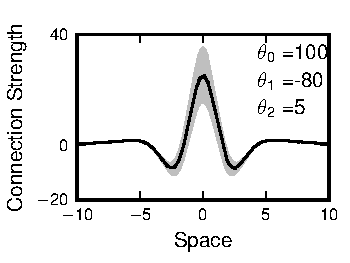
\includegraphics[height=6cm]{./Figures/Figure10a.pdf}
	\end{center}	
\end{frame}

\begin{frame}\frametitle{Monte Carlo simulation results - state estimation}
	\begin{center}
		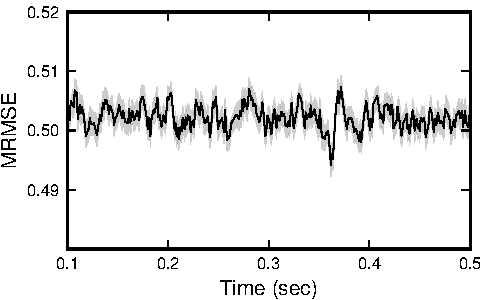
\includegraphics[height=6cm]{./Figures/fig8.pdf}
	\end{center}	
\end{frame}

\begin{frame} \frametitle{Field reconstruction}
	A movie was here
% \begin{center}
% \frame{\movie[height=154pt,width=311pt,poster,autoplay,repeat]{}{./Figures/FieldComparison.mov}}
% \end{center}
\end{frame}

\section[Recent Extensions]{Recent Extensions}

\begin{frame}\frametitle{Unknown Connectivity Kernel Support (and Isotropy)}

	\begin{center}
		\includegraphics<1>[height=6cm]{./Figures/KernelBasis1.pdf}
		\includegraphics<2>[height=6cm]{./Figures/KernelConvergence.pdf} 
		\includegraphics<3>[height=4cm]{./Figures/KernelEstimateCrossSection.pdf}  	
	\end{center}
	% \begin{picture}(0,0)
	% 	\put(120,20){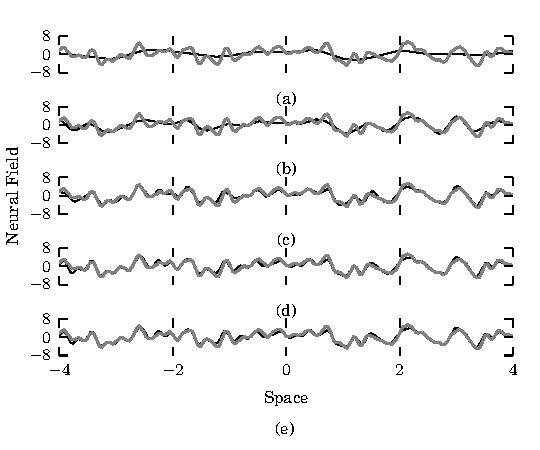
\includegraphics[height=5cm]{./Figures/MRAIDEfig1.pdf}}
	% 	\put(80,-100){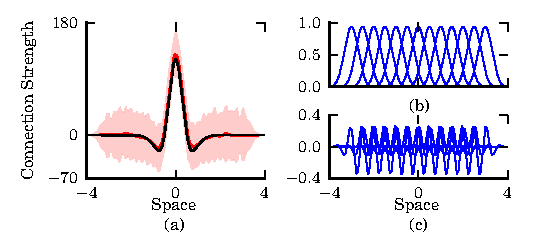
\includegraphics[height=4cm]{./Figures/MRAIDEfig2.pdf}}
	% \end{picture}
\end{frame}

\begin{frame}\frametitle{Unknown `Noise' Characteristics}

	\begin{center}
		\includegraphics<1>[height=6cm]{./Figures/DisturbanceWidthTrue.pdf}
		\includegraphics<2>[height=6cm]{./Figures/DisturbanceWidthEstimationBinary.pdf}
		\includegraphics<3>[height=3cm]{./Figures/Histogram.pdf}  	
	\end{center}
\end{frame}

\begin{frame}\frametitle{Multi-resolution}

	\begin{center}
		\includegraphics<1>[height=6cm]{./Figures/MRAIDEfig1.pdf}
		\includegraphics<2>[height=4cm]{./Figures/MRAIDEfig2.pdf}	
	\end{center}
\end{frame}

\section[Summary and Discussion]{Summary and Discussion}

\begin{frame}\frametitle{Summary and Discussion}
	\begin{itemize}
		\item Recap
		\item Assumptions
		\item Future work
	\end{itemize}
	\begin{center}
		\includegraphics<1>[height=6cm]{./Figures/StimulationSeizureControl.pdf}
		\includegraphics<2>[height=6cm]{./Figures/BrainElectrode.pdf} 
		\includegraphics<3->[height=4.5cm]{./Figures/Columns.pdf}
		\begin{picture}(0,0)
			\put(-130,-115){\tiny Photo: Ecole Polytechnique Federale de Lausanne, HPC photo gallery, \emph{Golden Pyramids in Columns}}
		\end{picture}
		\includegraphics<3->[height=.5cm]{./Figures/WhiteSpace.pdf}
		\includegraphics<3->[height=4.5cm]{./Figures/Anatomy.pdf}	
	\end{center}
	% \begin{picture}(0,0)
	% 	\put(120,20){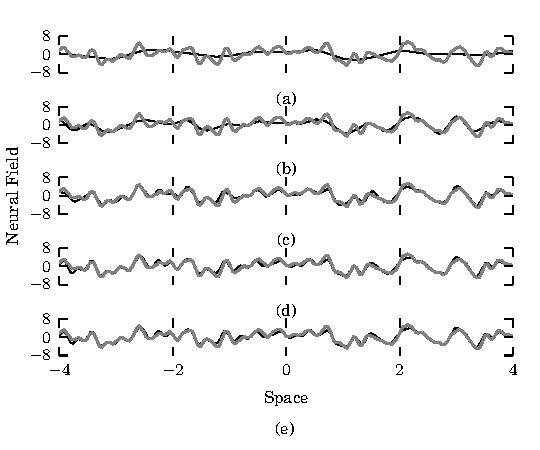
\includegraphics[height=5cm]{./Figures/MRAIDEfig1.pdf}}
	% 	\put(80,-100){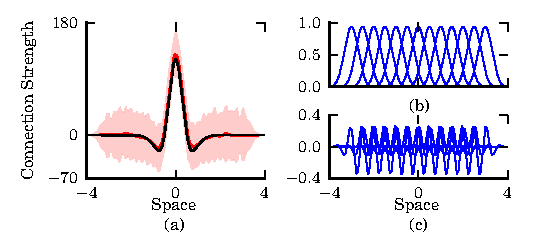
\includegraphics[height=4cm]{./Figures/MRAIDEfig2.pdf}}
	% \end{picture}
\end{frame}

\begin{frame}\frametitle{Patient-specific modelling - drug therapy}
	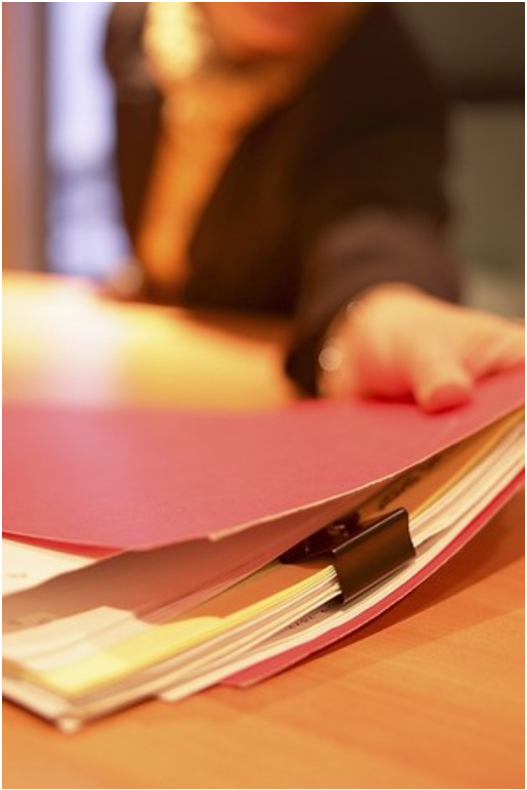
\includegraphics[height=5cm]{./Figures/PatientHistory.pdf}
	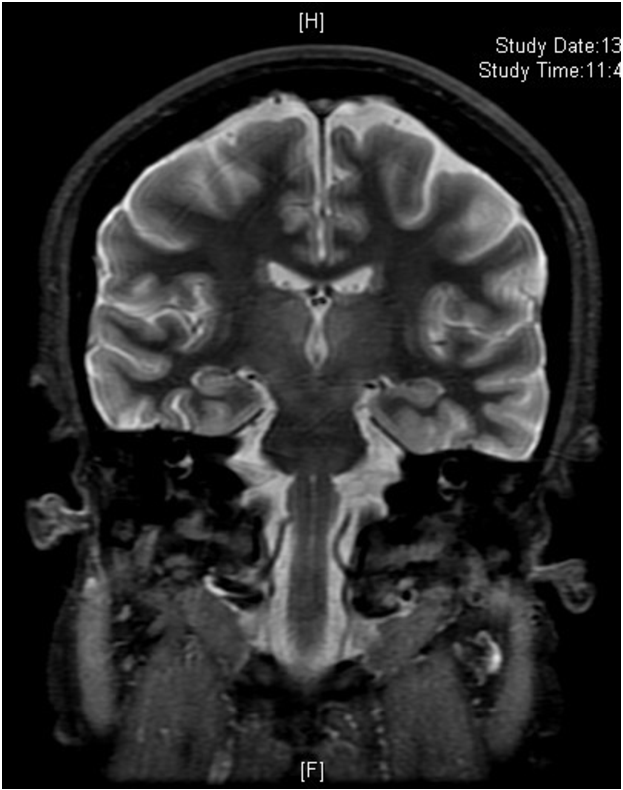
\includegraphics[height=5cm]{./Figures/PatientMRI.pdf}
	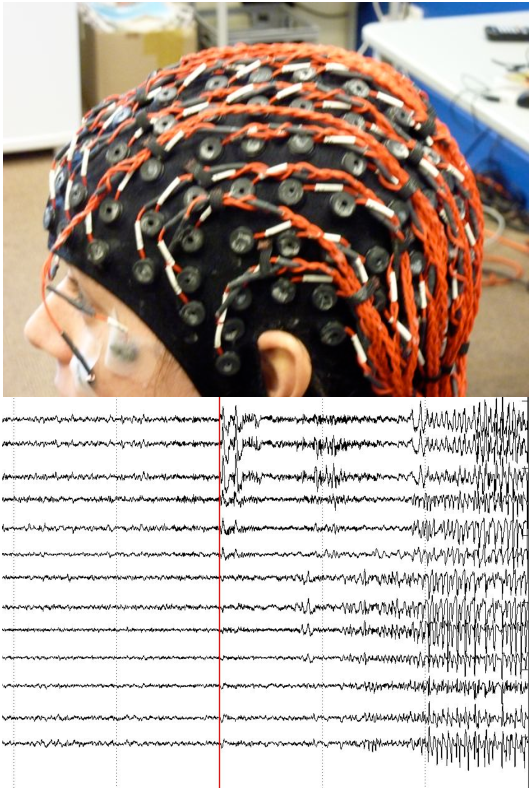
\includegraphics[height=5cm]{./Figures/PatientEEG.pdf}
\end{frame}
\begin{frame}\frametitle{That's it}
\begin{center}
	\large{Thanks!}
\end{center}
\end{frame}
\end{document}
